\documentclass[11pt,letterpaper]{article}

\usepackage[margin=1.5in]{geometry}
\usepackage[english]{babel}
\usepackage[utf8]{inputenc}
\usepackage{amsmath}
\usepackage{amssymb}
\usepackage{amsthm}
% IEEEtrantools (in the course template) is omitted here so the document compiles on minimal TeX installs; add it if you use IEEE-style equation stacks.
\usepackage{graphicx}
\usepackage{tabularx}
\usepackage{caption}
\usepackage{subfig}
% Course template uses kpfonts; fall back to Latin Modern if kpfonts is not installed.
\IfFileExists{kpfonts.sty}{\usepackage{kpfonts}}{\usepackage{lmodern}}
\usepackage{microtype}
\usepackage{booktabs}
\usepackage{bm}
\usepackage{listings}
\usepackage{verbatim}
\usepackage{xcolor}
\usepackage{mathtools}
\usepackage{setspace}
\usepackage{tikz}
\usepackage{float}
\usepackage{natbib}
\usepackage[colorlinks=true,linkcolor=blue,citecolor=blue,urlcolor=blue]{hyperref}
% \usepackage[colorinlistoftodos]{todonotes}  % optional; enable if todonotes is installed (course template)

\usetikzlibrary{arrows.meta, positioning, calc}

\newtheorem{definition}{Definition}
\newtheorem{proposition}{Proposition}
\newtheorem{theorem}{Theorem}
\newtheorem{corollary}{Corollary}

\singlespacing

\title{\textbf{Lobbying, Corruption, and Contagion on Council Networks}\\{\small \textbf{A Literature Review}}}
\author{Bryce Roberts  \and Samir Kadariya \\[0.5em]
\small 14.18 Mathematical Economic Modeling \quad|\quad MIT, Spring 2026}
\date{April 10, 2026}

\begin{document}

\maketitle

\begin{abstract}
This survey asks how an outside lobbyist can influence a networked council and what features of the council make such influence easier or harder. It reviews three related papers: \citet{shleifer1993} on the economics of corruption, \citet{galeotti2020} on optimal interventions in network games, and \citet{morris2000} on contagion in local interaction systems. Taken together, these papers suggest a common framework in which bribery changes legislators' private incentives, network spillovers amplify targeted intervention, and contagion determines whether influence remains local or becomes system-wide. The survey ends with three research questions on optimal targeting, contagion, and voting-rule design.
\end{abstract}

\section*{Introduction}

Consider a lobbyist who wants to pass a bill through a council. Council members are connected by party ties, committee overlap, and personal relationships, so influencing one member may also affect others. This makes lobbying a network problem as well as a corruption problem.

This review studies the following three papers:
\begin{itemize}
    \item \citet{shleifer1993}, which develops the economics of corruption;
    \item \citet{galeotti2020}, which studies optimal targeting in networks;
    \item \citet{morris2000}, which studies contagion in local interaction games.
\end{itemize}

\citet{shleifer1993} explain why bribes change incentives and why the organization of corruption matters. \citet{galeotti2020} explain how a strategic intervention is amplified by network structure. \citet{morris2000} explain when behavior spreads through a network rather than remaining local. More broadly, these papers fit into the literature on social and economic networks discussed by \citet{jackson2008}. By comparing these three models, the review studies how bribery, network position, and contagion fit together in a model of lobbying on council networks.

The rest of the paper proceeds as follows. Section~\ref{sec:sv} reviews \citet{shleifer1993}. Section~\ref{sec:ggg} reviews \citet{galeotti2020}. Section~\ref{sec:morris} reviews \citet{morris2000}. Section~\ref{sec:synth} presents a simple model suggested by these papers. Section~\ref{sec:concl} ends with three open questions.

\section{Shleifer and Vishny (1993): Corruption}
\label{sec:sv}

\subsection{Model}

\citet{shleifer1993} define government corruption as ``the sale by government officials of government property for personal gain.'' Their key insight is that corrupt officials can be modeled as monopolists. Officials control permits, licenses, contracts, or other government goods, and they can extract bribes by restricting supply in the same way that a monopolist restricts output to raise price.

In the simplest case, a single official controls one government good with demand curve $D(p)$. The official price is $\bar{p}$, but the official can create scarcity and charge an additional bribe. The official therefore behaves like a seller with market power over a government service that citizens or firms need in order to complete some economic activity. This is the basic monopoly analogy at the center of the paper.

The paper distinguishes two cases:

\begin{itemize}
    \item \textbf{Without theft.} The official remits the official price $\bar{p}$ to the government and keeps only the bribe. The effective marginal cost is therefore $\bar{p}$, and the official behaves like a tax collector who creates a shortage to maximize rents.
    \item \textbf{With theft.} The official hides the sale entirely and keeps both the official price and the bribe. The effective marginal cost falls to zero, making corruption even more attractive and harder to detect because no official record is created.
\end{itemize}

This distinction matters because it separates the incentive to bribe from the informational problem created by secrecy. In the without-theft case, corruption looks like a hidden tax layered on top of the official price. In the with-theft case, the official may even prefer to lower the buyer's total payment if that makes concealment easier, because the relevant objective is not public revenue but private extraction. Figure~\ref{fig:corruption} illustrates the case without theft: the official creates a shortage at the official price and extracts a bribe equal to the gap between the total price paid and $\bar{p}$.

\begin{figure}[t]
\centering
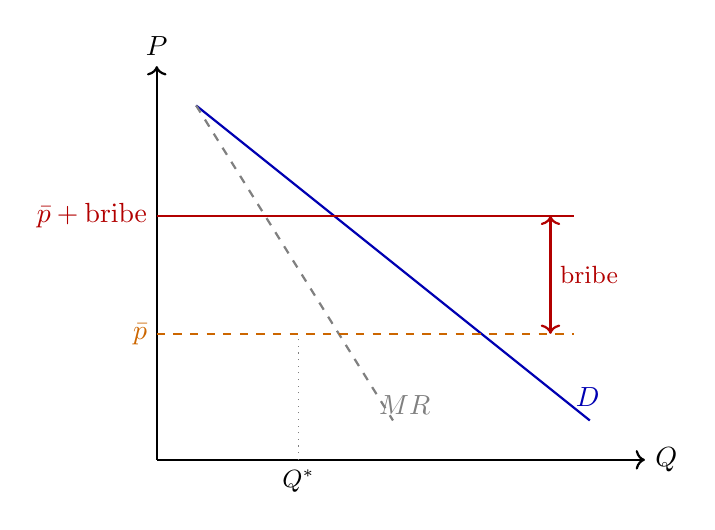
\begin{tikzpicture}[scale=1.0]
    \begin{scope}
    \draw[->, thick] (0,0) -- (6.2,0) node[right] {$Q$};
    \draw[->, thick] (0,0) -- (0,5.0) node[above] {$P$};
    \draw[thick, blue!70!black] (0.5,4.5) -- (5.5,0.5);
    \node[blue!70!black, right] at (5.2,0.8) {$D$};
    \draw[thick, gray, dashed] (0.5,4.5) -- (3.0,0.5);
    \node[gray, right] at (2.7,0.7) {$MR$};
    \draw[thick, orange!80!black, dashed] (0,1.6) -- (5.3,1.6);
    \node[left, orange!80!black] at (0,1.6) {$\bar{p}$};
    \draw[thick, red!70!black] (0,3.1) -- (5.3,3.1);
    \node[left, red!70!black] at (0,3.1) {$\bar{p}+\text{bribe}$};
    \draw[thick, red!70!black, <->] (5.0,1.6) -- (5.0,3.1);
    \node[right, red!70!black, font=\small] at (5.0,2.35) {bribe};
    \draw[dotted, gray] (1.8,0) -- (1.8,1.6);
    \node[below, font=\small] at (1.8,0) {$Q^*$};
    \end{scope}
\end{tikzpicture}
\caption{Corruption without theft. The official sets marginal revenue equal to the official price $\bar{p}$ and extracts a bribe on top, raising the total price to $\bar{p} + \text{bribe}$ and restricting output to $Q^*$. Adapted from \citet{shleifer1993}, Figure~Ia.}
\label{fig:corruption}
\end{figure}

\subsection{Main Results}

The paper becomes especially relevant in settings requiring several complementary government approvals, where officials might collude to maximize joint rents or act as independent extractors. A firm may need permits from multiple agencies to operate, meaning the total bribe burden depends on the network of corruption across those agencies. Let $x_1$ and $x_2$ denote quantities of two complementary government goods. The core idea is that if a buyer needs several approvals at once, each agency's bribe affects the demand faced by the others.

\medskip
\noindent \textbf{Joint monopoly (centralized corruption).} If one organization internalizes all bribe revenue, it recognizes that a higher bribe on one approval lowers demand for the other. The optimality condition is
\begin{equation}
    MR_1 + MR_2 \frac{dx_2}{dx_1} = MC_1,
    \label{eq:joint-monopoly}
\end{equation}
so with complementary goods the joint monopolist sets a lower effective bribe than separate agencies would. This is the least damaging corrupt regime from the payer's perspective because complementarities are internalized.

\medskip
\noindent \textbf{Independent monopolists (decentralized corruption).} If each agency maximizes its own bribe revenue, it ignores the effect of its price on the demand faced by the other agency. Relative to \eqref{eq:joint-monopoly}, each office effectively sets the cross-effect to zero, so bribes are higher and output is lower.

\medskip
\noindent \textbf{Competition.} If several non-colluding agencies can supply the same approval, competition drives bribes toward zero.



\medskip
The central result is that decentralized corruption is worse than centralized corruption for both buyers and aggregate output. This structural outcome depends heavily on the officials' mutual awareness and capacity to collude. When officials know the full set of required approvals and can coordinate their rent extraction, they effectively form a centralized monopoly. This collusive structure internalizes the cross-elasticity of demand, leading to a lower equilibrium bribe that preserves some level of aggregate activity. However, when officials are unaware of one another or cannot sustain collusion, the system fractures into an anti-commons problem: each isolated agency imposes its own toll without accounting for how that toll reduces total activity. Their well-known example is post-Soviet Russia, where foreign investors needed approvals from multiple siloed ministries, each demanding a localized bribe. The result was not simply redistribution, but a collapse in investment driven by a structural coordination failure.

The paper also emphasizes secrecy. Corruption must be hidden, so resources are shifted toward transactions where side payments are easier to conceal. This is one reason the authors argue that corruption is often more distortionary than taxation: it not only raises private costs, but also reallocates activity toward less transparent forms of exchange.

\subsection{Conclusion and Discussion}

This paper provides the economic motivation for the topic. It explains why a bribe can change a decision maker's incentives and how the structural organization of corruption—specifically, the degree of awareness and collusion among officials—dictates the equilibrium level of rent extraction. It also suggests two themes that are useful later in the review: first, corruption depends inherently on how decision makers are linked and what information they share; and second, secrecy matters because influence is not fully observable. However, while Shleifer and Vishny rely on a binary distinction between complete collusion (centralization) and complete independence (decentralization), their model lacks a formal network structure. It cannot answer how specific, localized linkages affect the broader equilibrium, which official should be targeted first, or whether corruption can spread contagiously through a partially connected group. The next paper studies this network side of the problem.
\section{Galeotti, Golub, and Goyal (2020): Targeting Interventions in Networks}
\label{sec:ggg}

\subsection{Model}

\citet{galeotti2020} study a simultaneous-move game on a network. Agent $i$ chooses a continuous action $a_i \in \mathbb{R}$, and payoffs depend on both private incentives and neighbors' actions:
\begin{equation}
    U_i(\mathbf{a}, \mathbf{G}) = a_i \left( b_i + \beta \sum_j g_{ij} a_j \right) - \frac{1}{2} a_i^2,
    \label{eq:ggg-payoff}
\end{equation}
where $\mathbf{G}$ is a weighted adjacency matrix, $b_i$ is the agent's standalone return, and $\beta$ captures whether actions are strategic complements or substitutes. The best response is
\begin{equation}
    a_i = b_i + \beta \sum_j g_{ij} a_j,
    \label{eq:ggg-best-response}
\end{equation}
and, when $\mathbf{G}$ is symmetric and the spectral radius of $\beta \mathbf{G}$ is below one, the unique equilibrium is
\begin{equation}
    \mathbf{a}^* = [\mathbf{I} - \beta \mathbf{G}]^{-1} \mathbf{b}.
    \label{eq:ggg-equilibrium}
\end{equation}

The planner in their model shifts the vector of standalone returns from a status quo $\hat{\mathbf{b}}$ to a new vector $\mathbf{b}$ subject to a quadratic budget constraint. The planner chooses this intervention before agents move and then evaluates outcomes using utilitarian welfare. It is helpful to think of this intervention as changing how willing each agent is to act before strategic spillovers begin. The planner therefore does not directly choose actions; instead, the planner changes the environment in which actions are chosen.

The continuous-action setup is useful because it separates two objects clearly. The vector $\mathbf{b}$ describes the direct incentive each agent has to act. The matrix $\mathbf{G}$ describes how each person's action affects the incentives of others. This makes it possible to ask whether an intervention should target agents with strong direct incentives, agents in important network positions, or both.

This separation is one reason the paper is easy to apply in other settings. For example, one can imagine $b_i$ as a student's desire to study, a firm's incentive to invest, or a politician's willingness to support a bill. The network then captures how each person's behavior affects those around them. In each case, the same formal model can be used to ask how an outside intervention changes the final equilibrium.

\subsection{Main Results}

Because $\mathbf{G}$ is symmetric, it can be diagonalized as $\mathbf{G} = \mathbf{U}\boldsymbol{\Lambda}\mathbf{U}^{\top}$. Writing \eqref{eq:ggg-equilibrium} in the principal-component basis gives
\begin{equation}
    \underline{a}^*_{\ell} = \frac{1}{1 - \beta \lambda_{\ell}} \underline{b}_{\ell},
    \label{eq:ggg-component}
\end{equation}
where $\lambda_{\ell}$ is the $\ell$th eigenvalue of $\mathbf{G}$ and $\underline{b}_{\ell}$ is the projection of $\mathbf{b}$ onto the corresponding eigenvector. The term $(1 - \beta \lambda_{\ell})^{-1}$ is the network multiplier for component $\ell$: it measures how strongly the network amplifies an intervention aligned with that component.

This principal-component representation is one of the main ideas of the paper. Instead of thinking about the network one link at a time, the paper rewrites the problem in terms of a few large directions of variation. Each principal component is a pattern of behavior over the whole network. Some patterns are amplified a lot by strategic spillovers, and some are amplified only weakly. The planner therefore cares not only about which agent to target, but also about which broad pattern of intervention the network makes most effective.

The main theorem in \citet{galeotti2020} characterizes the optimal intervention in terms of its similarity to the principal components of the network. In words, the planner should intervene most strongly in the directions that the network amplifies the most. Three implications are especially important:

\begin{enumerate}
    \item \textbf{Strategic complements.} When actions are complements, the optimal intervention is tilted toward the first principal component, so central agents receive more weight.
    \item \textbf{Strategic substitutes.} When actions are substitutes, the intervention tilts toward the last principal component, reflecting the network's more oppositional structure.
    \item \textbf{Spectral gap.} The difference between the leading eigenvalues determines how simple the optimal intervention is. A large spectral gap makes the targeting rule close to one-dimensional; a small gap forces the planner to spread resources across several directions.
\end{enumerate}

These three points can be read in a very intuitive way. Under complements, helping an already central agent has a large indirect effect because their action feeds back through many others. Under substitutes, concentrating intervention on the same type of agent is less useful, so the planner instead chooses a more balancing pattern. The spectral gap matters because it tells us whether there is one clearly dominant way to intervene or several competing ones.

The budget also matters. With a small budget, the status quo remains important and the intervention is typically complex. With a large budget, the network's dominant component matters more. In the complements case, the optimal intervention approaches eigenvector centrality as the budget grows. In the substitutes case, the intervention instead reflects the network's most oppositional or bipartite structure. Figure~\ref{fig:spectral-gap} illustrates this contrast.

This distinction between small and large budgets shows that network targeting is not just about identifying one ``most central'' individual. When resources are limited, the planner still has to pay attention to the baseline profile $\hat{\mathbf{b}}$ and to how several principal components interact. When resources are abundant, the network itself plays a larger role and the intervention becomes much simpler.

It is also useful to compare this result to a simpler intuition that one might have before reading the paper. A natural guess is that the planner should always target the agents with the highest centrality. Galeotti, Golub, and Goyal show that this is not always true. It becomes approximately true in some high-budget complements settings, but in general the best intervention depends on the kind of strategic spillovers, the baseline profile, and the full spectrum of the network.

\begin{figure}[t]
\centering
\subfloat[Cohesive network: large spectral gap\label{fig:spectral-cohesive}]{
\begin{minipage}{0.47\textwidth}
\centering
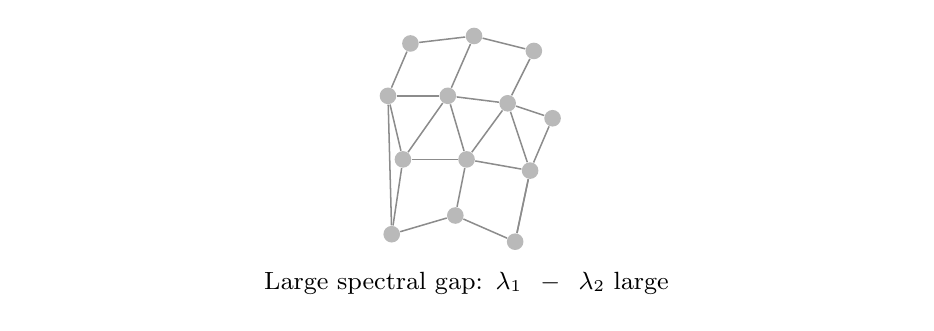
\begin{tikzpicture}[scale=0.95,
    nd/.style={circle, fill=gray!55, minimum size=6pt, inner sep=0pt},
    ndh/.style={circle, fill=gray!55, minimum size=6pt, inner sep=0pt}]
    \node[nd] (a1) at (0,0) {};
    \node[nd] (a2) at (0.85,0.25) {};
    \node[ndh] (a3) at (1.65,-0.1) {};
    \node[nd] (a4) at (0.15,1.0) {};
    \node[ndh] (a5) at (1.0,1.0) {};
    \node[nd] (a6) at (1.85,0.85) {};
    \node[nd] (a7) at (-0.05,1.85) {};
    \node[ndh] (a8) at (0.75,1.85) {};
    \node[nd] (a9) at (1.55,1.75) {};
    \node[nd] (a10) at (2.15,1.55) {};
    \node[nd] (a11) at (0.25,2.55) {};
    \node[ndh] (a12) at (1.1,2.65) {};
    \node[nd] (a13) at (1.9,2.45) {};
    \foreach \i/\j in {a1/a2,a2/a3,a4/a5,a5/a6,a7/a8,a8/a9,a9/a10,a11/a12,a12/a13,a1/a4,a2/a5,a3/a6,a4/a7,a5/a8,a6/a9,a7/a11,a8/a12,a9/a13,a4/a8,a5/a9,a6/a10,a1/a7,a3/a6} {
        \draw[black!45, line width=0.55pt] (\i)--(\j);
    }
    \node[font=\small, text width=0.9\linewidth, align=center] at (1.0,-0.65) {Large spectral gap: $\lambda_1 - \lambda_2$ large};
\end{tikzpicture}
\end{minipage}
}
\hfill
\subfloat[Fragmented network: small spectral gap\label{fig:spectral-frag}]{
\begin{minipage}{0.47\textwidth}
\centering

\begin{tikzpicture}[scale=0.95,
    nd/.style={circle, fill=gray!55, minimum size=6pt, inner sep=0pt},
    ndh/.style={circle, fill=gray!55, minimum size=6pt, inner sep=0pt}]
    \node[nd] (L1) at (0,0.25) {};
    \node[ndh] (L2) at (0.55,0) {};
    \node[nd] (L3) at (0.35,0.85) {};
    \node[ndh] (L4) at (0.9,0.65) {};
    \node[nd] (L5) at (0.1,1.55) {};
    \node[nd] (L6) at (0.65,1.45) {};
    \node[ndh] (L7) at (0.4,2.1) {};
    \foreach \i/\j in {L1/L2,L2/L4,L3/L4,L3/L5,L5/L6,L6/L7,L1/L3,L4/L6} {
        \draw[black!45, line width=0.55pt] (\i)--(\j);
    }
    \node[ndh] (R1) at (2.0,0.25) {};
    \node[nd] (R2) at (2.55,0) {};
    \node[ndh] (R3) at (2.35,0.85) {};
    \node[nd] (R4) at (2.9,0.65) {};
    \node[nd] (R5) at (2.1,1.55) {};
    \node[ndh] (R6) at (2.65,1.45) {};
    \node[nd] (R7) at (2.4,2.1) {};
    \foreach \i/\j in {R1/R2,R2/R4,R3/R4,R3/R5,R5/R6,R6/R7,R1/R3,R4/R6} {
        \draw[black!45, line width=0.55pt] (\i)--(\j);
    }
    \draw[black!75, line width=1.1pt] (L4) -- (R3);
    \node[font=\small, text width=0.9\linewidth, align=center] at (1.45,-0.65) {Small spectral gap: $\lambda_1 - \lambda_2$ small};
\end{tikzpicture}
\end{minipage}
}
\caption{Stylized council networks and the spectral gap. Panel~(a) depicts a densely connected council: interventions can align with a dominant principal component, so the optimal targeting rule is relatively simple. Panel~(b) depicts two communities linked by a thin bridge: the planner must balance resources across competing parts of the network, so the optimal intervention blends several components.}
\label{fig:spectral-gap}
\end{figure}

\subsection{Conclusion and Discussion}

This paper is useful because it shows how a targeted intervention is amplified by a network. In the council setting considered here, a bribe can be interpreted as a shift in a member's standalone incentive. The paper does not study corruption directly, and its planner is benevolent rather than adversarial, but it gives the basic network machinery for thinking about whom a lobbyist should target and how a council's structure affects the answer.

At the same time, the paper does not answer every question needed for the lobbying setting. It studies continuous actions rather than a final yes-or-no vote, and it studies how actions respond in equilibrium rather than whether a small change can spread through the network over time. For that reason, the next paper is useful as a complement. It addresses a different question: even if an initial target is well chosen, when does that local change spread through the whole network?

\section{Morris (2000): Contagion}
\label{sec:morris}

\subsection{Model}

\citet{morris2000} study a local interaction game on an infinite network. Each player chooses one action to play against all neighbors, and best responses depend on the fraction of neighbors taking each action. Formally, a local interaction system is a triple $(\chi,\sim,q)$, where $\chi$ is a countably infinite set of players, $\sim$ is a symmetric neighborhood relation, and $q \in (0,1)$ is a payoff parameter. Each neighboring pair plays the coordination game
\begin{equation}
\begin{array}{c|cc}
 & 0 & 1 \\
\hline
0 & q, q & 0, 0 \\
1 & 0, 0 & 1-q, 1-q
\end{array}.
\label{eq:morris-game}
\end{equation}
A player switches to action 1 when at least a fraction $q$ of neighbors choose 1.

\begin{definition}[Contagion threshold]
The \textit{contagion threshold} $\xi$ of a local interaction system $(\chi,\sim)$ is the largest $q$ such that action 1 spreads by best-response dynamics from some finite initial group to the whole population.
\end{definition}

The paper also distinguishes contagion from uninvadability. An action is contagious if a small initial set can spread it through the whole population. An action is uninvadable if, once almost everyone plays it, a small set of deviators cannot overturn it. These are closely related but distinct ideas: one concerns diffusion from a seed, and the other concerns resistance to reversal.

This framework captures a different margin than \citet{galeotti2020}. Galeotti, Golub, and Goyal study how targeted intervention changes equilibrium actions in a continuous game, while Morris studies when a local shock causes a discrete cascade. For lobbying on council networks, both margins matter.

\subsection{Main Results}

\citet{morris2000} show that contagion depends sharply on network geometry:

\begin{itemize}
    \item \textbf{Line.} If players are arranged on $\mathbb{Z}$ and each has two neighbors, then $\xi = \frac{1}{2}$.
    \item \textbf{$m$-dimensional lattice.} With nearest-neighbor interaction on $\mathbb{Z}^m$, the threshold is $\xi = \frac{1}{2m}$.
    \item \textbf{Regions.} If cliques of size $m$ are arranged in a line, then $\xi = \frac{1}{m+1}$.
    \item \textbf{Hierarchy.} In a tree with branching factor $m$, the threshold is also $\xi = \frac{1}{m+1}$.
\end{itemize}

The striking lesson is that more links do not automatically make contagion easier. Richer local neighborhoods often raise the number of supporting neighbors required for switching, so dense connectivity can inhibit cascades rather than promote them. Figure~\ref{fig:morris-topologies} visualizes this comparison: a line can spread with a thinner local base than a richer grid. A council that is easy to target in the sense of \citet{galeotti2020} need not be easy to tip into full contagion in the sense of \citet{morris2000}.

\begin{figure}[t]
\centering
\subfloat[Line network\label{fig:morris-line}]{
\begin{minipage}{0.47\textwidth}
\centering
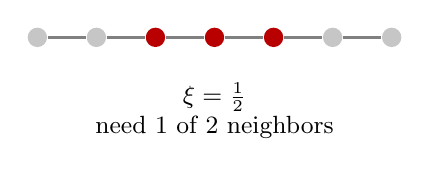
\begin{tikzpicture}[scale=1.0,
    nd/.style={circle, fill=gray!45, minimum size=7pt, inner sep=0pt},
    hot/.style={circle, fill=red!72!black, minimum size=7pt, inner sep=0pt}]
    \node[nd] (n0) at (0,0) {};
    \node[nd] (n1) at (0.75,0) {};
    \node[hot] (n2) at (1.5,0) {};
    \node[hot] (n3) at (2.25,0) {};
    \node[hot] (n4) at (3.0,0) {};
    \node[nd] (n5) at (3.75,0) {};
    \node[nd] (n6) at (4.5,0) {};
    \draw[black!50, line width=0.9pt] (n0) -- (n1) -- (n2) -- (n3) -- (n4) -- (n5) -- (n6);
    \node[below, font=\small, align=center] at (2.25,-0.45) {$\xi = \frac{1}{2}$\\need 1 of 2 neighbors};
\end{tikzpicture}
\end{minipage}
}
\hfill
\subfloat[Grid network (2D lattice)\label{fig:morris-grid}]{
\begin{minipage}{0.47\textwidth}
\centering
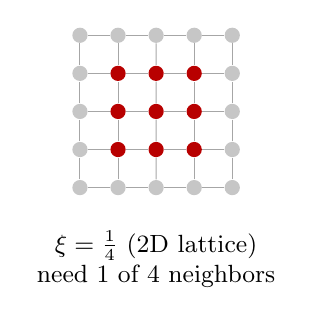
\begin{tikzpicture}[scale=0.78,
    nd/.style={circle, fill=gray!45, minimum size=5.5pt, inner sep=0pt},
    hot/.style={circle, fill=red!72!black, minimum size=5.5pt, inner sep=0pt}]
    \foreach \x in {0,...,4} {
        \foreach \y in {0,...,4} {
            \pgfmathparse{(\x>=1 && \x<=3 && \y>=1 && \y<=3) ? 1 : 0}
            \ifnum\pgfmathresult=1
                \node[hot] (g\x\y) at (\x*0.62,\y*0.62) {};
            \else
                \node[nd] (g\x\y) at (\x*0.62,\y*0.62) {};
            \fi
        }
    }
    \foreach \x in {0,...,4} {
        \foreach \y [evaluate=\y as \ny using int(\y+1)] in {0,...,3} {
            \draw[black!35, line width=0.35pt] (g\x\y) -- (g\x\ny);
        }
    }
    \foreach \y in {0,...,4} {
        \foreach \x [evaluate=\x as \nx using int(\x+1)] in {0,...,3} {
            \draw[black!35, line width=0.35pt] (g\x\y) -- (g\nx\y);
        }
    }
    \node[below, font=\small, align=center] at (1.24,-0.55) {$\xi = \frac{1}{4}$ (2D lattice)\\need 1 of 4 neighbors};
\end{tikzpicture}
\end{minipage}
}
\caption{Stylized topology comparison for \citet{morris2000}. Red nodes highlight an initial cluster of adopters. On a line, each interior player has two neighbors; on the square grid, interior players have four. Morris's thresholds imply that the same fraction $q$ can require more supporting neighbors in absolute terms when degree is higher, which is one reason denser local structure need not make contagion easier.}
\label{fig:morris-topologies}
\end{figure}

Morris's more general contribution is to replace case-by-case topology arguments with a structural concept: cohesion. Let $\pi[X|x]$ be the share of player $x$'s neighbors who belong to group $X$.

\begin{definition}[$p$-cohesion]
A group $X$ is \textit{$p$-cohesive} if every member of $X$ has at least proportion $p$ of their interactions within the group.
\end{definition}

Highly cohesive groups are natural firewalls. If members mostly interact with one another, outside behavior has difficulty crossing the threshold needed to induce switching. The tightest internal roadblock in the network therefore limits how far a local shock can spread. Morris also connects contagion to broader structural properties such as low neighbor growth and $\delta$-uniformity, which together explain why some locally dense and homogeneous networks support stronger contagion than others.

In a legislature, factions, parties, or committees may function as cohesive blocs. A lobbyist may influence one member and still fail to trigger broader support if nearby blocs are tight enough to resist cascade dynamics. This is a useful lesson for this topic because it shows that contagion depends not just on how many links a council has, but on how those links are organized.

\citet{morris2000} also clarify why spreading a convention differs from spreading information. \citet{granovetter1973} famously argued that weak ties help information travel across groups, but Morris shows that convention change requires local reinforcement. A legislator is unlikely to switch political support after seeing one isolated neighbor move; switching is more plausible when enough trusted neighbors move together. This distinction matters here because lobbying influence may spread like a convention rather than like a piece of information: repeated local reinforcement can matter more than sheer reach.

\subsection{Conclusion and Discussion}

Morris is useful for this topic because it explains when local influence spreads and when it does not. The paper does not include a strategic intervener, but it tells us how network structure and local cohesion shape the possibility of contagion. Together with \citet{galeotti2020}, it helps separate two questions that are easy to confuse: who should be targeted, and whether that targeting will generate a cascade. This distinction is useful in a council setting, where the most central member is not necessarily the member from whom a majority cascade is easiest to generate.

\section{A Simple Model}
\label{sec:synth}

Taken together, the three papers suggest a simple research framework with three stages, illustrated in Figure~\ref{fig:timing}. A lobbyist chooses transfers $\mathbf{t} = (t_1,\ldots,t_n)$ across council members subject to a budget $\sum_i t_i \leq B_L$. Council members then choose support levels $a_i$ on a network $\mathbf{G}$. The bill passes if aggregate support exceeds a threshold.

\begin{figure}[t]
\centering
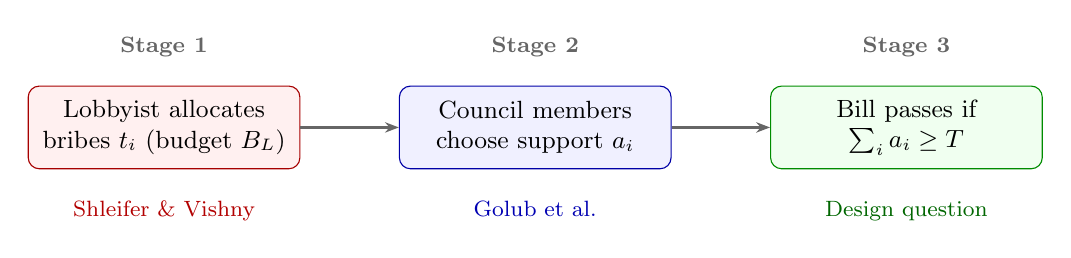
\begin{tikzpicture}[
    box/.style={rectangle, draw=black!65, fill=gray!6, rounded corners=4pt,
        text=black, font=\small, minimum width=3.45cm, minimum height=1.05cm, align=center},
    arr/.style={-{Stealth[length=5pt]}, thick, black!60},
    stage/.style={font=\footnotesize\bfseries, text=black!60},
    src/.style={font=\footnotesize, text=black!75}
]
    \node[box, draw=red!65!black, fill=red!6] (s1) {Lobbyist allocates\\bribes $t_i$ (budget $B_L$)};
    \node[box, draw=blue!65!black, fill=blue!6, right=1.25cm of s1] (s2) {Council members\\choose support $a_i$};
    \node[box, draw=green!55!black, fill=green!6, right=1.25cm of s2] (s3) {Bill passes if\\$\sum_i a_i \geq T$};
    \draw[arr] (s1) -- (s2);
    \draw[arr] (s2) -- (s3);
    \node[stage, above=7pt] at (s1.north) {Stage 1};
    \node[stage, above=7pt] at (s2.north) {Stage 2};
    \node[stage, above=7pt] at (s3.north) {Stage 3};
    \node[src, below=8pt, text=red!70!black] at (s1.south) {Shleifer \& Vishny};
    \node[src, below=8pt, text=blue!70!black] at (s2.south) {Golub et al.};
    \node[src, below=8pt, text=green!40!black] at (s3.south) {Design question};
\end{tikzpicture}
\caption{Timing of the lobbying model. The bribe allocation draws on the corruption logic of \citet{shleifer1993}, the simultaneous support game uses the network framework of \citet{galeotti2020}, and the passage threshold motivates the institutional design question. The contagion analysis of \citet{morris2000} governs whether localized support cascades across the network in Stage~2.}
\label{fig:timing}
\end{figure}

A reduced-form payoff for legislator $i$ is
\begin{equation}
U_{i}=a_{i}(b_{i}+t_{i}+\beta\sum_{j}g_{ij}a_{j})-\frac{1}{2}ca_{i}^{2},
\end{equation}
where $b_{i}$ is the legislator's baseline inclination toward the bill, $t_{i}$ is the private transfer, $\beta>0$ captures strategic complementarities such as political cover, persuasion, or reputational alignment, and $c>0$ represents the marginal cost of exerting political support. Under the same stability logic as in \citet{galeotti2020}, the equilibrium is
\begin{equation}
    \mathbf{a}^* = [c\mathbf{I} - \beta \mathbf{G}]^{-1}(\mathbf{b} + \mathbf{t}).
    \label{eq:lobbying-equilibrium}
\end{equation}

This section is meant to describe a starting point rather than a finished theory. The goal is not to claim that the three papers already solve the lobbying problem once they are put together. Instead, the goal is to write down one simple model that draws one key idea from each paper and shows how the ideas might be combined in later work.

The first idea comes from \citet{shleifer1993}. The transfer term $t_i$ represents the basic idea that an outside payment can change a decision maker's incentives. The second idea comes from \citet{galeotti2020}. The network term $\beta \sum_j g_{ij} a_j$ says that one council member's support affects others through social or political ties. The third idea comes from \citet{morris2000}. Although the equation above is continuous, the model can later be connected to a binary voting or contagion setting by asking when higher support levels are large enough to produce a cascade.

One way to read the model is as follows. The term $b_i$ captures whether legislator $i$ already likes or dislikes the bill. The term $t_i$ captures how lobbying changes that direct incentive. The network term captures peer effects: a legislator may find it easier to support a bill when allies, party members, or close collaborators are also supporting it. The threshold stage then connects these support choices to an institutional outcome, namely whether the bill passes.

This starting model keeps the later research questions in view. Once the model is written down, one can ask which member should receive the largest transfer, whether support spreads beyond the initially targeted members, and whether the voting threshold makes the council more or less resistant to outside influence. The model is included only to organize the ideas from the three papers and to show where the next research step would begin.

\section{Open Questions}
\label{sec:concl}

The three papers raise the following open questions:
\begin{itemize}
    \item How does the network structure of a council affect the lobbyist's optimal bribery strategy and the equilibrium level of support for a bill?
    \item Under what conditions does bribing one council member cause support for the bill to spread contagiously through the network?
    \item What voting rule---majority, supermajority, or weighted voting---is most robust to outside lobbying, given the council's network structure?
\end{itemize}

\begingroup
\small
\setlength{\itemsep}{0pt}
\setlength{\parskip}{0pt}
\begin{thebibliography}{99}

\bibitem[Galeotti et al.(2020)Galeotti, Golub, and Goyal]{galeotti2020}
Galeotti, Andrea, Benjamin Golub, and Sanjeev Goyal. ``Targeting Interventions in Networks.'' \textit{Econometrica} 88, no. 6 (2020): 2445--2471.

\bibitem[Granovetter(1973)]{granovetter1973}
Granovetter, Mark S. ``The Strength of Weak Ties.'' \textit{American Journal of Sociology} 78, no. 6 (1973): 1360--1380.

\bibitem[Jackson(2008)]{jackson2008}
Jackson, Matthew O. \textit{Social and Economic Networks}. Princeton University Press, 2008.

\bibitem[Morris(2000)]{morris2000}
Morris, Stephen. ``Contagion.'' \textit{The Review of Economic Studies} 67, no. 1 (2000): 57--78.

\bibitem[Shleifer and Vishny(1993)]{shleifer1993}
Shleifer, Andrei, and Robert W. Vishny. ``Corruption.'' \textit{The Quarterly Journal of Economics} 108, no. 3 (1993): 599--617.

\end{thebibliography}
\endgroup

\end{document}
